\documentclass[main.tex]{subfiles}

\begin{document}

In order to use beta decay as a laboratory to find new physics, the current theory of beta decay must be discussed.
Beta decay ultimately originates from the standard model weak interaction.
The weak interaction is moderated by the nuclei.

\section{Beta Decay and the Weak Interaction}
The underlying process of $e_{-}$ beta decay at the quark level is a down quark going into an up quark plus an electron plus an anti-electron neutrino.
For positron decay, the process is an up quark going to a down quark plus a positron plus an electron neutrino. 
This needs to be described using an effective field theory lagrangian. 

\section{Matrix elements of Beta Decay}
When the beta decay rate is calculated, there are several terms.
There are phase space terms, which originate from the density of states.
These and the electromagnetic interactions will be discussed further into the thesis. 
The contribution to beta decay $M$ from the weak interaction, to first order, is shown in equation \ref{eq:decayrate} \cite{ref:oscarpaper}

\begin{equation}
	M = \xi [1 + a \frac{\vec{p_{e}} \dot \vec{p_{\nu}}} {E_{e} E_{\nu}}  +  b \frac{m_{e}}{E_{e}} + \frac{\vec{<J>}}{J} \dot (A \frac{ \vec{p_{e}} }{E_{e}} + B \frac{\vec{p_{\nu}}}{E_{\nu}} + D \frac{\vec{p_{e}} \times \vec{p_{\nu}}}{E_{e} E_{\nu}})]
	\label{eq:decayrate}
\end{equation}
where $\xi$ is a constant that depends, to first order, on the Lee-Yang coupling constants, $\vec{p}$  is the momentum of either the electron $e$ or the neutrino $\nu$, and $E$ the energy of the same particle.
$<\vec{J}>$ is the average total angular momentum. 
The constants $a$, $b$, $A$, $B$, and $D$ can be written in terms of the coupling constants as well.
$a$ depends on the mixing of the Gamow-Teller and Fermi matrix elements.
A polarized nucleus is need to extract $a$. 
For an unpolarized beam where only the energy of the electron is measured, the momenta are averaged over and all terms disappear expect for $b$.
This term is known as the Fierz term, and a measurement of the Fierz term was the ultimate goal of this experiment. 

\section{Fierz Term}
The Fierz term, $b$, in equation \ref{eq:decayrate}, can be rewritten in terms of effective couplings.
This is shown in equation \ref{eq:bwrittenout}

\begin{equation}
	b =  \pm \sqrt{1 - \alpha^{2}{Z^{2}}}\frac{1}{1 + \rho}Re(\frac{C_{S} + C_{S}'}{C_{V} + C_{V}'} + |\rho|^{2}\frac{C_{T} + C_{T}'}{C_{A} + C_{A}'})
	\label{eq:bwrittenout}
\end{equation}

where $\rho$ is the ratio of the Gamow-Teller matrix element to Fermi matrix element, $\alpha$ is the QED fine structure constant \cite{OSCARPAPER}. 
The subscripts of $C$ indicate which object the coupling corresponds to. 
Here, $A$ means axial vector, $V$ stands for polar vector, $S$ stands for scalar, and $T$ stands for tensor. 
The $C$ coefficients correspond to parity conserving interactions, and the $C'$ coefficents correspond to parity non-conserving coefficents \cite{Lee56}
This means, that in a pure Fermi decay, the Fierz term is sensitive to any non-standard scalar term, while in a pure Gamow-Teller decay, the Fierz term is sensitive to any non-standard Tensor terms. 
The Fermi decays have been measured using super-allowed beta decays, where the spin change is $0^{+}$ to $0^{+}$. 
In order to get a good measurement of any tensor couplings, an allowed Gamow-Teller decay must be used. 

\section{$^{20}$F Decay}
In order to get a measurement of the Fierz term, a nucleus that beta decays is needed.
In this measurement, the nucleus used was $^{20}$F.
The decay scheme is given in figure \ref{fig:DecayScheme}.

\begin{figure}[!htb]
	\centerline{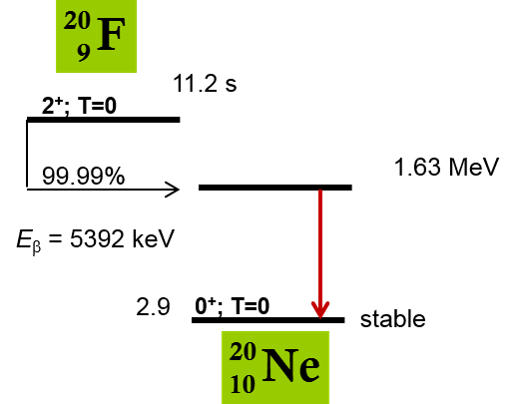
\includegraphics[width=0.78\textwidth]{20FDecayScheme.png}}
	\caption{The decay scheme of $^{20}$F.}
	\label{fig:DecayScheme}
\end{figure}

As seen in the figure, $^{20}$F decays 99.999\% of the time to the first excited state of $^{20}$Ne.
The $2^{+}$ state seen in the decay scheme is not the isobaric analogue state to the ground state of $^{20}$F.
That state is much higher in energy.
The beta decay therefor has a isospin change of 1, and is a Gamow-Teller transition.
The higher order matrix elements are very small.
This means the Fierz term is sensitive to potential tensor couplings.
The half-life of $^{20}$F is about 11 seconds. 
This is an important consideration for the experimental design.
The gamma ray and the end point energy of the electron are also important for the experimental design.
In order to get at the Fierz term, the beta decay spectrum shape must be described percisely.
The next chapter deals with the corrections to the beta decay spectrum.  

\end{document}